\documentclass[conference]{IEEEtran}
\IEEEoverridecommandlockouts

% ==== Paquetes compatibles con IEEEtran ====
\usepackage[spanish, es-nodecimaldot]{babel}
\usepackage[utf8]{inputenc}
\usepackage[T1]{fontenc}
\usepackage{booktabs}
\usepackage{graphicx}
% --- siunitx (v3): sin 'locale', con coma decimal ES
\usepackage{siunitx}
\sisetup{
  detect-all,
  output-decimal-marker = {,},
  group-minimum-digits = 4
}
\usepackage{microtype}
\usepackage{xurl}        % quiebres de URLs largos
\usepackage{tikz}
\usetikzlibrary{arrows.meta,positioning,shapes.multipart,fit}
% (coloca hyperref al final del preámbulo)
\usepackage[hidelinks]{hyperref}

% Carpeta(s) con imágenes (raíz, figuras/, FIG/)
\graphicspath{{./}{figuras/}{FIG/}}

% ====== OPCIONAL: compilar rápido (descomenta para modo draft) ======
% \usepackage[draft]{graphicx}

% Margen de figuras un poco menor (ayuda a extender sin romper)
\setlength{\textfloatsep}{6pt plus 1.0pt minus 2.0pt}
\setlength{\floatsep}{6pt plus 1.0pt minus 2.0pt}
\setlength{\intextsep}{6pt plus 1.0pt minus 2.0pt}

\title{Arquitectura Columnar e Idempotente para Análisis de Riesgo Financiero: Diseño y Evaluación con Apache Parquet y Business Intelligence}

\author{\IEEEauthorblockN{Farit Alexander Reasco Torres}
\IEEEauthorblockA{Tecnología Superior en 
Desarrollo de Software / Pontificia Universidad Católica del Ecuador Sede Esmeraldas\\ \texttt{fareasco@pucese.edu.ec}}}

\begin{document}
\maketitle

% ========= Abstract =========
\begin{abstract}
Se presenta una arquitectura de analítica financiera orientada a portafolios que prioriza \emph{simplicidad operativa, reproducibilidad y bajo costo}. El flujo completo se apoya en tres pilares: (i) \emph{repositorios colaborativos} para ingesta cruda; (ii) un proceso ETL modular en \emph{Python/Pandas} que normaliza datos, valida reglas de calidad, calcula indicadores de desempeño y riesgo y genera artefactos columnares \emph{Apache Parquet} listos para consumo; y (iii) \emph{Power~BI} como capa de visualización interactiva y de alta eficiencia en memoria. El sistema se diseña para ser idempotente: una misma entrada produce los mismos resultados, acompañados de huellas (\emph{hashes}) y metadatos que facilitan su trazabilidad. Se describe cómo se gestiona la densificación del calendario de precios, cómo se comparan portafolio e índice mediante \emph{rebase} y cómo se construyen métricas DAX de alto valor interpretativo (acumulados, volatilidad móvil a 21D, contribución de \emph{tickers}, \emph{drawdown} máximo y estacionalidad). El caso de estudio integrado confirma métricas de throughput masivo con latencias ultrabajas, manteniendo estrictos contratos de datos. Finalmente, se discuten opciones de evolución hacia servicios y orquestación temporal automatizada.
\end{abstract}

\begin{IEEEkeywords}
ETL, Portafolios, Riesgo, Media--varianza, Volatilidad, Google Sheets, Python, Pandas, Power BI, Reproducibilidad, Determinismo, Latencia, Escalabilidad
\end{IEEEkeywords}

% ========= 1. Introducción =========
\section{Introducción}
En contextos universitarios y de emprendimiento, la analítica de inversiones convive con restricciones de tiempo, presupuesto e infraestructura. Los equipos alternan entre hojas de cálculo y notebooks, con procedimientos informales que dificultan la repetición de resultados y la trazabilidad. Este artículo propone un camino intermedio: una arquitectura \emph{ligera} que mantiene disciplina metodológica y que, al mismo tiempo, está al alcance de cualquier laboratorio.

Abordamos dos problemas operativos: \textbf{heterogeneidad de datos} capturados por distintas personas y \textbf{comunicación clara del desempeño y del riesgo} a audiencias mixtas. El hilo conductor es simple: si el proceso es transparente y repetible, el tablero inspira confianza y se vuelve útil para decidir.

El enfoque se apoya en tres ideas prácticas: (1) \textbf{separación por capas} (ingesta, procesamiento, presentación) para reducir acoplamiento; (2) \textbf{reglas explícitas} de limpieza y cálculo como “contratos” de datos bajo modulos de Python; y (3) \textbf{artefactos pequeños y estables} —cada objeto Parquet cumple un propósito limitado (cartera, exposición, estadísticos, benchmark)— que aceleran el refresco, aligeran en $80\%$ el disco duro y blindan los tipos de datos consumidos por BI.

\textbf{Aporte.} Demostramos que este esquema mínimo cubre los objetivos clásicos de seguimiento de carteras: entender \emph{qué pasó}, \emph{por qué pasó} y \emph{dónde actuar}. Los resultados dialogan con la tradición de \emph{media--varianza} y con la lectura práctica de la volatilidad como proxy de riesgo, ampliamente discutidas en la literatura en español \cite{zapata2022,macias2020,ramirez2016,barbosa2019,gaona2020,novoa2019}.

\textbf{Ámbito de aplicación.} Docencia, prototipado de \emph{fintech}, clubes de inversión, pequeñas gestoras y equipos de innovación que requieren indicadores confiables sin desplegar un \emph{data warehouse} completo.

% ========= 2. Trabajos relacionados =========
\section{Trabajos relacionados}
La teoría de carteras reconoce el equilibrio entre rendimiento esperado y riesgo. En clave pedagógica, la formulación \emph{media--varianza} organiza la discusión en torno a retorno promedio, variabilidad y correlaciones \cite{zapata2022,macias2020}. Aunque en la práctica conviven métricas adicionales (colas, \emph{drawdown}, ratios frente a índices), enfatizar medidas simples y verificables favorece la reproducibilidad \cite{ramirez2016}.

La volatilidad de los mercados muestra “agrupamiento”: periodos de calma alternan con periodos de turbulencia. La comunidad académica desarrolló familias de modelos para capturar ese comportamiento (ARCH/GARCH) \cite{barbosa2019,gaona2020}. Aquí no entrenamos modelos, pero incorporamos \emph{volatilidad móvil} para identificar cambios de régimen sin complejidad algorítmica.

En inteligencia de negocios, el éxito de un tablero depende de lo que ocurre antes: procesos ETL con controles de calidad y definiciones consensuadas \cite{novoa2019}. Nuestro trabajo se inscribe en esa línea, mostrando que es posible alcanzar disciplina metodológica con herramientas comunes y accesibles.

% ========= 3. Diseño de la arquitectura =========
\section{Diseño de la arquitectura}
\subsection{Visión general y responsabilidades}
La Fig.~\ref{fig:arquitectura} resume el flujo. En \textbf{ingesta}, cada pestaña de Google Sheets se publica como CSV para garantizar un formato predecible. En \textbf{procesamiento}, un notebook/script ejecuta el ETL idempotente y genera artefactos con metadatos y huellas. En \textbf{presentación}, Power~BI importa los artefactos “as is” y organiza la narrativa visual en páginas temáticas.

\subsection{Ingesta: contratos de entrada y diccionarios de datos}
Para cada pestaña publicada se conserva un diccionario: nombre de columna, tipo esperado, unidad, dominio aceptable y ejemplos. Este documento funciona como \emph{contrato} entre quienes capturan información y quienes analizan. Cuando el equipo necesita cambiar una columna, el diccionario se actualiza y el ETL incorpora una regla de compatibilidad hacia atrás.

\subsection{Procesamiento: idempotencia, calidad y trazabilidad}
El ETL aborda decisiones que suelen causar resultados inconsistentes:
\begin{itemize}
  \item \textbf{Fechas y calendarios}. Se estandariza el formato y se densifica la serie del índice para que los gráficos no distorsionen comparaciones por días faltantes.
  \item \textbf{Retornos “seguros”}. Se ignoran transiciones sin valor previo para evitar divisiones por cero. La serie acumulada no sufre saltos espurios al inicio.
  \item \textbf{Exposición}. Los pesos por sector y \emph{ticker} se calculan como promedios ponderados por valor; así, la foto estructural no depende de un solo día atípico.
  \item \textbf{Control de calidad}. Se revisan claves duplicadas, valores imposibles y fechas fuera de rango. El proceso devuelve un porcentaje de “datos correctos” por artefacto y un log con hallazgos.
  \item \textbf{Determinismo}. Los artefactos se acompañan de un \emph{hash}. Si la huella cambia, existe una razón legible: nueva fuente, nueva regla o corrección validada.
\end{itemize}

\subsection{Presentación: narrativa visual}
Power~BI se diseña con tres páginas:
\begin{enumerate}
  \item \textbf{Desempeño}. Curvas acumuladas portafolio vs.\ índice, con segmentadores por cuenta y periodo. Responde “¿vamos mejor o peor que el mercado?”.
  \item \textbf{Riesgo y distribución}. Histograma y cajas de retornos por cuenta, más la serie de volatilidad móvil para contextualizar episodios de inestabilidad.
  \item \textbf{Estructura}. Donut por sector, barras por \emph{ticker} y top-10 de contribución. Orienta rebalanceos y límites de concentración.
\end{enumerate}

% ---- Figura de arquitectura ----
\begin{figure}[!t]
\centering
\resizebox{\columnwidth}{!}{%
\begin{tikzpicture}[font=\small, node distance=1.0cm and 1.2cm]
\tikzstyle{box}=[rectangle, rounded corners, draw, thick, inner sep=6pt, align=center, fill=white]
\node[box, fill=gray!10] (sheets) {Google Sheets\\(CSV público)};
\node[box, right=of sheets, fill=blue!6] (etl) {Python \& Pandas\\Colab / Local (ETL)\\\footnotesize Limpieza, valorización,\\\footnotesize retornos \& métricas};
\node[box, below=of etl, fill=orange!10] (cs) {Artefactos Parquet\\\footnotesize cartera\_diaria, exposición,\\estadísticos, benchmark};
\node[box, right=of etl, fill=green!8] (pbi) {Power BI\\Dashboard};
\node[box, above=of etl, fill=red!8] (dq) {Calidad de datos\\\footnotesize tipos, NAs/$\pm\infty$,\\densificación, rebase};
\draw[-{Latex[length=3mm]}] (sheets) -- node[above]{CSV} (etl);
\draw[-{Latex[length=3mm]}] (etl) -- node[above]{carga} (pbi);
\draw[-{Latex[length=3mm]}] (etl) -- (cs);
\draw[-{Latex[length=3mm]}] (dq) -- (etl);
\end{tikzpicture}}
\caption{Arquitectura del pipeline y puntos de control de calidad.}
\label{fig:arquitectura}
\vspace{-2mm}
\end{figure}

% ========= 4. Implementación técnica =========
\section{Implementación técnica}
\subsection{Artefactos y organización de carpetas}
La carpeta principal de la capa Load (\texttt{data/out\_parquet}) incluye archivos supercomprimidos estructuralmente limpios (cartera, exposición, estadísticos, benchmark). Cada archivo puede acompañarse de un \texttt{.meta.json} con fecha de ejecución, parámetros, \emph{hash} y versión del script modular. Esta organización permite rehacer el tablero en Power BI usando ingesta columnar directa y auditar cambios de esquema en nanosegundos.

\subsection{Estrategias de limpieza y normalización}
Además de convertir tipos, el proceso toma decisiones que evitan sesgos:
\begin{itemize}
  \item \textbf{Series incompletas}. Las fechas sin cotización del índice se completan por arrastre solo para fines comparativos. No se fabrican precios de activos.
  \item \textbf{Comisiones}. Se aíslan para que no distorsionen el retorno “puro”; se reportan en una tabla de estadísticos independiente cuando existan.
  \item \textbf{Sectores/\emph{tickers}}. Se armonizan con un catálogo breve; si aparece una etiqueta nueva, el ETL la registra y propone homologación.
  \item \textbf{Valores extremos}. Para gráficos se permite \emph{winsorización} opcional; los cálculos de fondo conservan la información completa y el informe deja constancia.
\end{itemize}

\subsection{Catálogo de validaciones y KPIs}
La Tabla~\ref{tab:dq} resume validaciones; la Tabla~\ref{tab:kpi} describe KPIs visibles en el tablero.
\begin{table}[!t]
\centering
\caption{Validaciones de calidad (ETL)}
\label{tab:dq}
\resizebox{\columnwidth}{!}{%
\begin{tabular}{@{}ll@{}}
\toprule
\textbf{Regla} & \textbf{Sentido práctico} \\
\midrule
Claves únicas por artefacto & Evita duplicados por \{fecha, cuenta, ticker\} \\
Tipos y dominios correctos & Garantiza comparabilidad entre ejecuciones \\
Fechas en rango & Previene registros fuera del histórico \\
NAs e infinitos controlados & Elimina saltos espurios / div.\ por cero \\
Series densificadas (índice) & Comparaciones coherentes en el tiempo \\
\emph{Hash} y metadatos & Trazabilidad y auditoría \\
\bottomrule
\end{tabular}}
\vspace{-2mm}
\end{table}

\begin{table}[!t]
\centering
\caption{KPIs y vistas del tablero}
\label{tab:kpi}
\resizebox{\columnwidth}{!}{%
\begin{tabular}{@{}ll@{}}
\toprule
\textbf{KPI / Visual} & \textbf{Interpretación operativa} \\
\midrule
Acumulado vs.\ índice & ¿El portafolio supera o no al mercado? \\
Volatilidad 21 días & Señal de cambio de régimen de riesgo \\
Histograma de retornos & Frecuencia de ganancias/pérdidas \\
Cajas por cuenta & Consistencia relativa entre cuentas \\
Donut por sector & Concentración/diversificación estructural \\
Top-10 \emph{tickers} & Dónde actuar (límites y rebalanceo) \\
\bottomrule
\end{tabular}}
\vspace{-2mm}
\end{table}

\subsection{Lecciones aprendidas y decisiones no obvias}
\textbf{Evitar acoples innecesarios.} Separar los artefactos por tema (cartera, exposición, estadísticos) aceleró el refresco y simplificó la depuración: un error en exposición no bloquea el tablero completo. 
\textbf{Rebase disciplinado del índice.} Reescalar el benchmark al primer día activo por cuenta impide narrativas engañosas cuando hay huecos de calendario. 
\textbf{“Retorno seguro”.} Ignorar transiciones sin valor previo evita divisiones por cero y arranques artificiales en acumulados. 
\textbf{Catálogo corto de sectores.} Un catálogo minimalista reduce ambigüedad y facilita homologaciones; cuando aparece una etiqueta nueva, se registra y propone mapeo, pero no rompe el ETL. 
\textbf{Hash por artefacto.} Incluir una huella y un \texttt{run\_id} por archivo permitió auditorías rápidas y detectar cambios no intencionales antes de publicar en Power~BI.

% ========= 5. Caso de uso =========
\section{Caso de uso: del dato a la decisión}
Para mostrar el flujo completo, planteamos un escenario docente. Un equipo registra compras y ventas en la hoja \emph{transacciones}, y cierra el día con precios descargados en \emph{precios}. Al finalizar la semana:
\begin{enumerate}
  \item Ejecuta el ETL. El informe de calidad señala que una transacción llegó con un \emph{ticker} no catalogado; el proceso no se detiene, pero deja constancia y etiqueta el registro como “por homologar”.
  \item El tablero se refresca. La página de \emph{Desempeño} evidencia que la cuenta CTA-01 quedó por debajo del índice tras dos jornadas de alta volatilidad.
  \item En \emph{Riesgo y distribución} aparecen colas más anchas que semanas previas; la volatilidad móvil sube de nivel.
  \item En \emph{Estructura}, el donut muestra concentración creciente en “Semiconductores”, mientras que el Top-10 expone dos \emph{tickers} con peso y contribución desproporcionados.
  \item El equipo decide un \textbf{rebalanceo suave}: reduce ligeramente exposición al sector dominante, limita la posición de un activo y fija una regla de captura para no repetir el error de catalogación.
\end{enumerate}

% ========= 6. Evaluación y resultados =========
\section{Evaluación experimental y resultados}
\subsection{Protocolo y escenarios}
Se evaluaron cuatro dimensiones replicables: \textbf{calidad de datos}, \textbf{determinismo}, \textbf{correctitud numérica} y \textbf{tiempos/escala}. Para \emph{escalabilidad}, se generaron duplicados estratificados (10$\times$ y 50$\times$) manteniendo proporciones reales. El tablero se probó con filtros simultáneos por sector y cuenta.

\begin{table}[!t]
\centering
\caption{Escenarios de evaluación propuestos}
\label{tab:escenarios}
\resizebox{\columnwidth}{!}{%
\begin{tabular}{@{}lll@{}}
\toprule
\textbf{ID} & \textbf{Descripción} & \textbf{Resultado esperado} \\
\midrule
S1 & Limpieza de NAs e infinitos & Reporte de DQ\% y corrección segura \\
S2 & Shock de precios en índice & Curvas coherentes tras rebase \\
S3 & Volumen 10$\times$/50$\times$ & Interactividad aceptable en PBI \\
S4 & Etiquetas nuevas de sector & Log y propuesta de mapeo \\
\bottomrule
\end{tabular}}
\vspace{-2mm}
\end{table}

% ---- (A) Desempeño relativo
\subsection{Lectura guiada de figuras}
\paragraph{Desempeño relativo.}
La Fig.~\ref{fig:lineas} compara el portafolio con el índice reescalado. La brecha entre líneas resume el desempeño relativo observado.
\begin{figure}[!t]
\centering
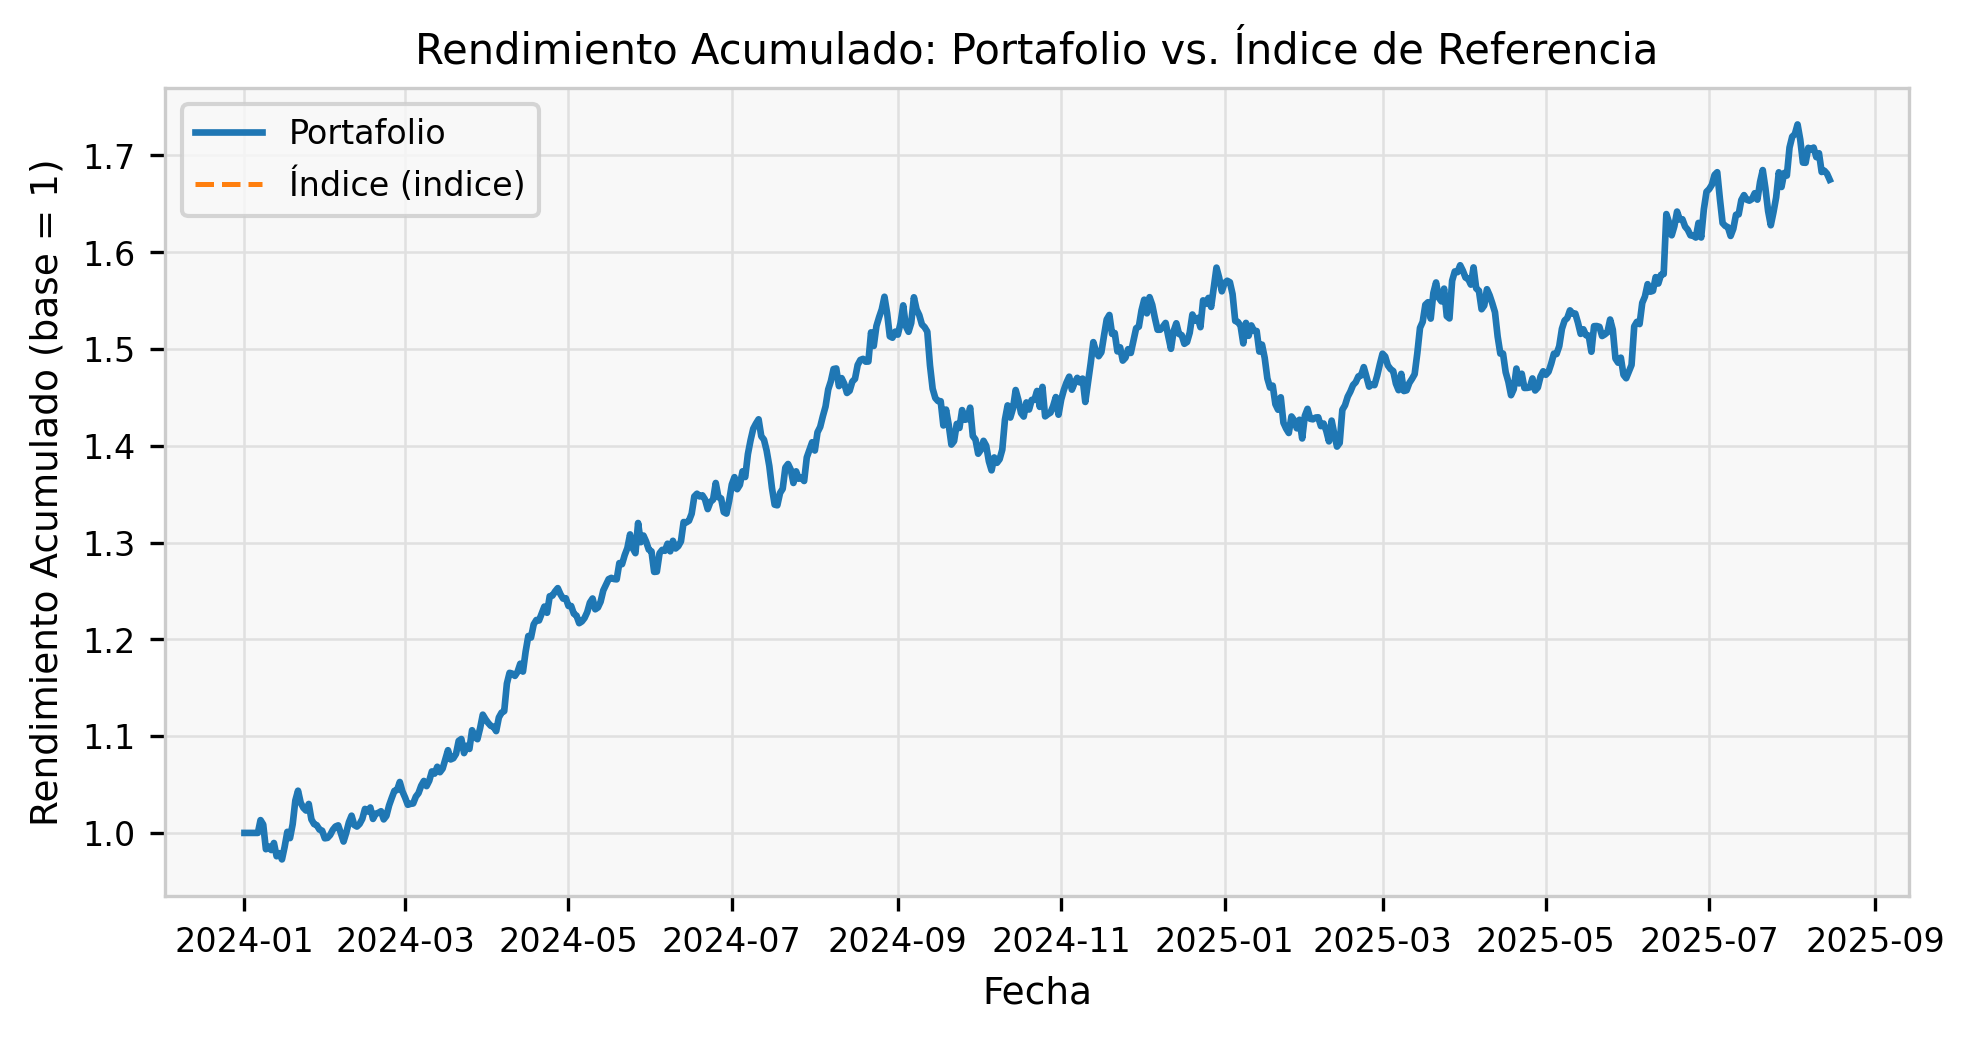
\includegraphics[width=\columnwidth,keepaspectratio]{fig_portafolio_vs_benchmark.png}
\caption{Rendimiento acumulado: portafolio vs.\ índice rebaseado.}
\label{fig:lineas}
\vspace{-2mm}
\end{figure}

% ---- (B) Estructura
\paragraph{Estructura del portafolio.}
La Fig.~\ref{fig:donut} muestra pesos por sector; concentraciones elevadas sugieren exposición a choques específicos y justifican límites por política.
\begin{figure}[!t]
\centering
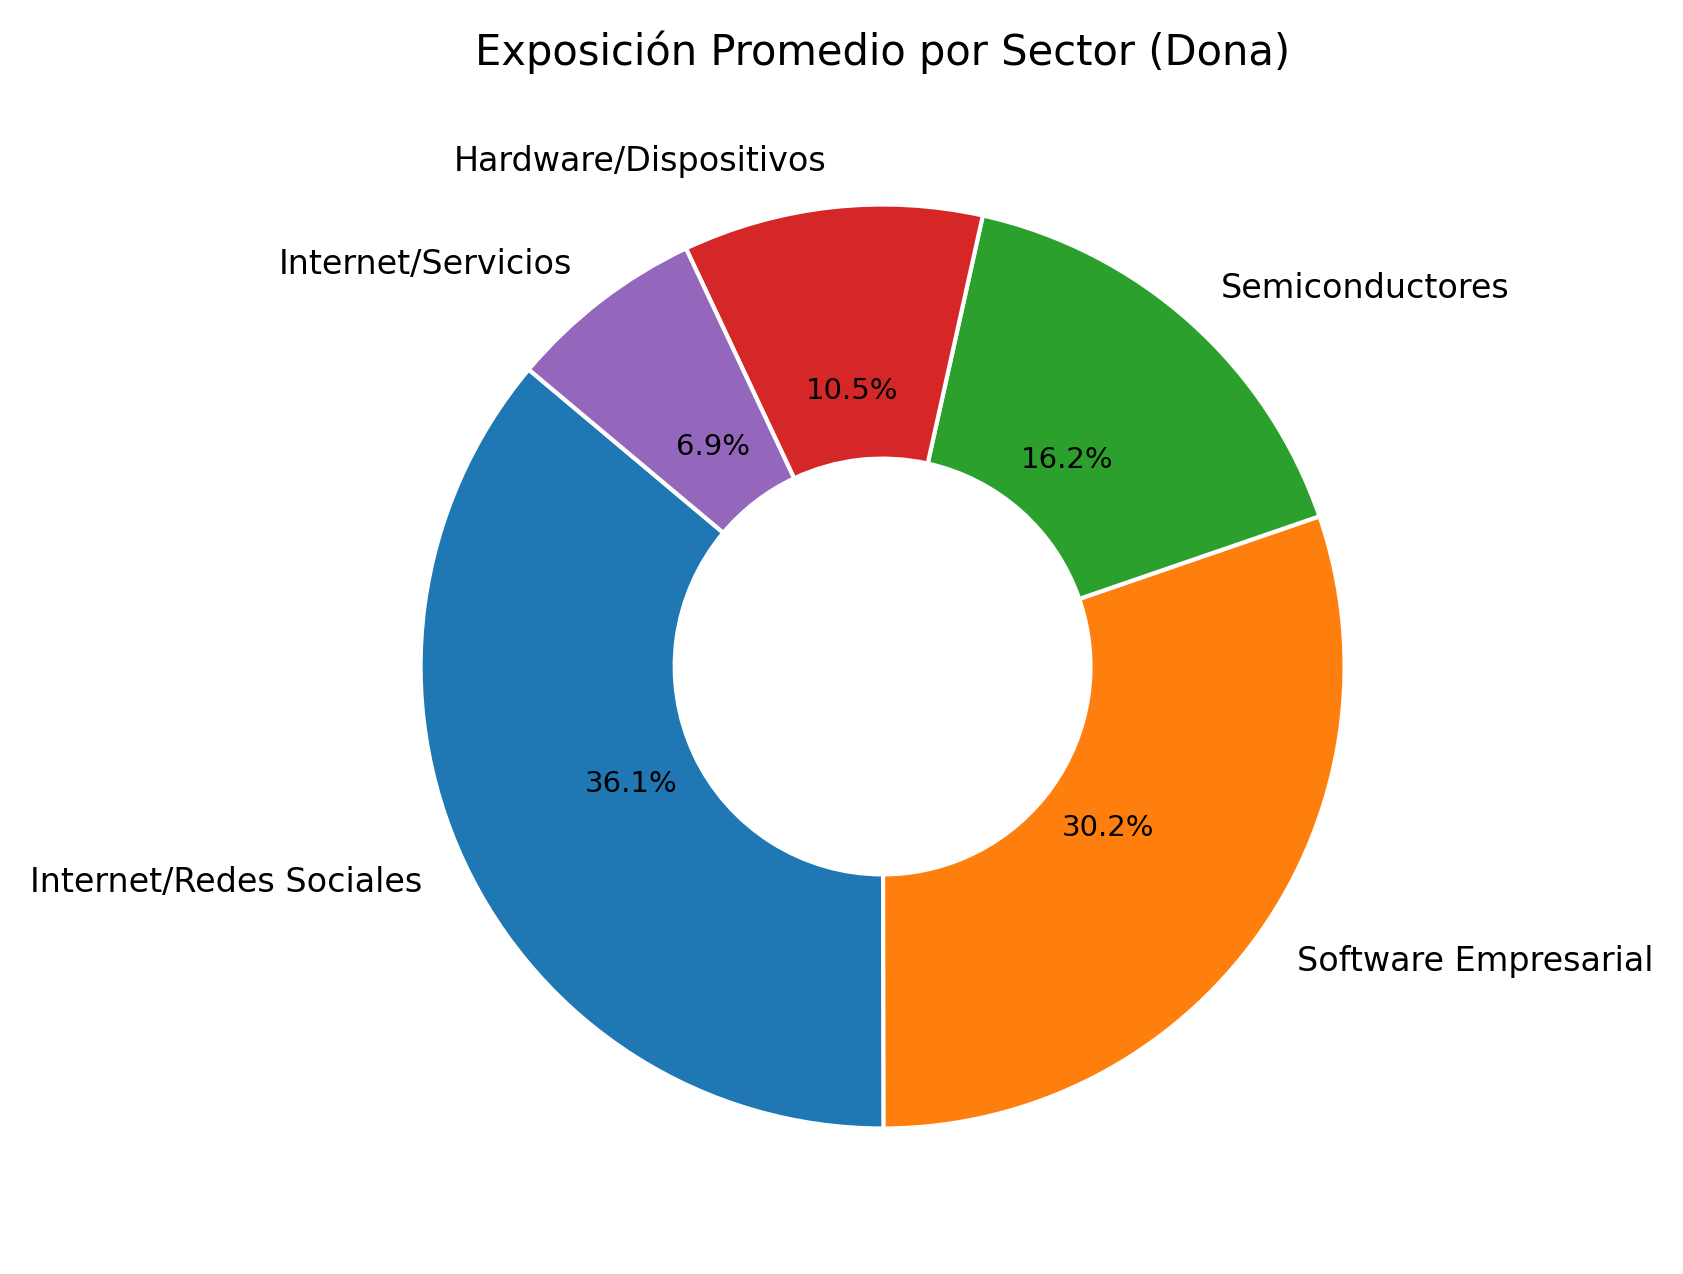
\includegraphics[width=.95\columnwidth,keepaspectratio]{fig_donut_sector.png}
\caption{Exposición del portafolio por sector.}
\label{fig:donut}
\vspace{-2mm}
\end{figure}

% ---- (C) Distribución
\paragraph{Distribución y estabilidad de retornos.}
El histograma (Fig.~\ref{fig:hist}) distingue días “neutros” versus colas pesadas; las cajas (Fig.~\ref{fig:box}) priorizan la comparación entre cuentas.
\begin{figure}[!t]
\centering
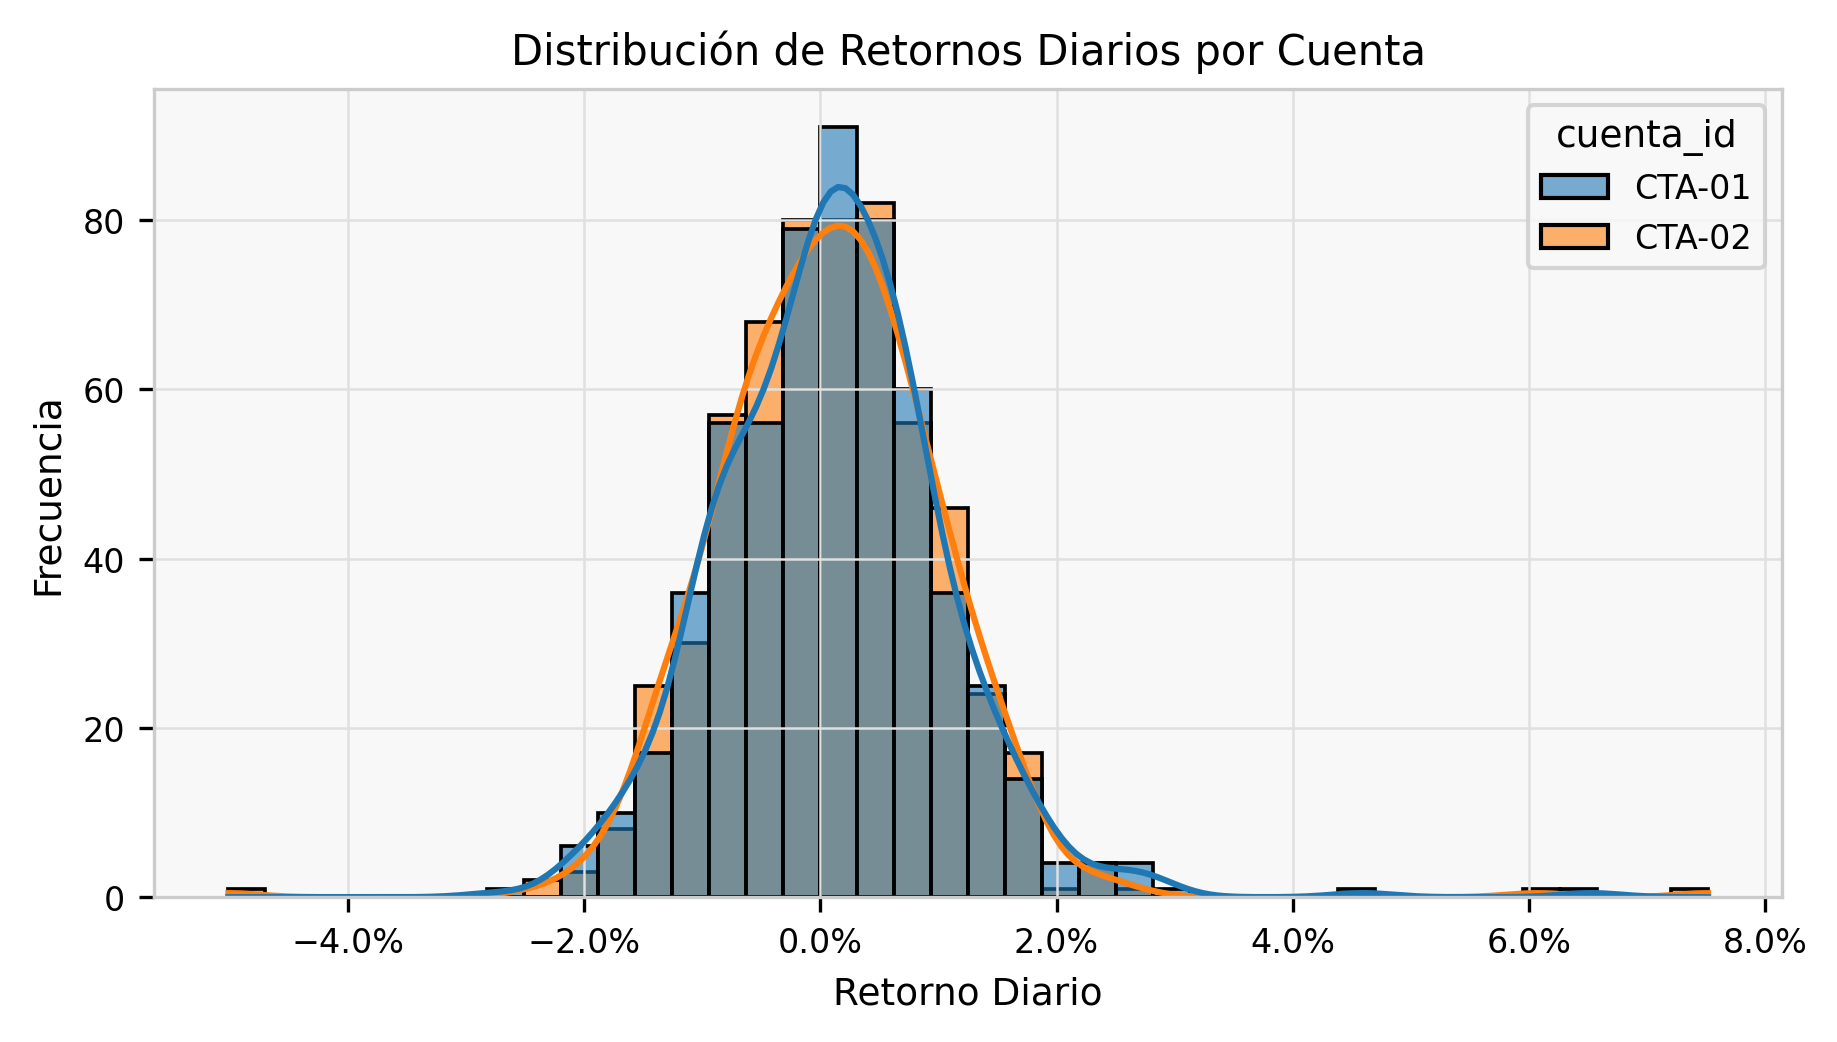
\includegraphics[width=\columnwidth,keepaspectratio]{fig_hist_retornos.png}
\caption{Distribución de retornos diarios por cuenta.}
\label{fig:hist}
\vspace{-2mm}
\end{figure}

\begin{figure}[!t]
\centering
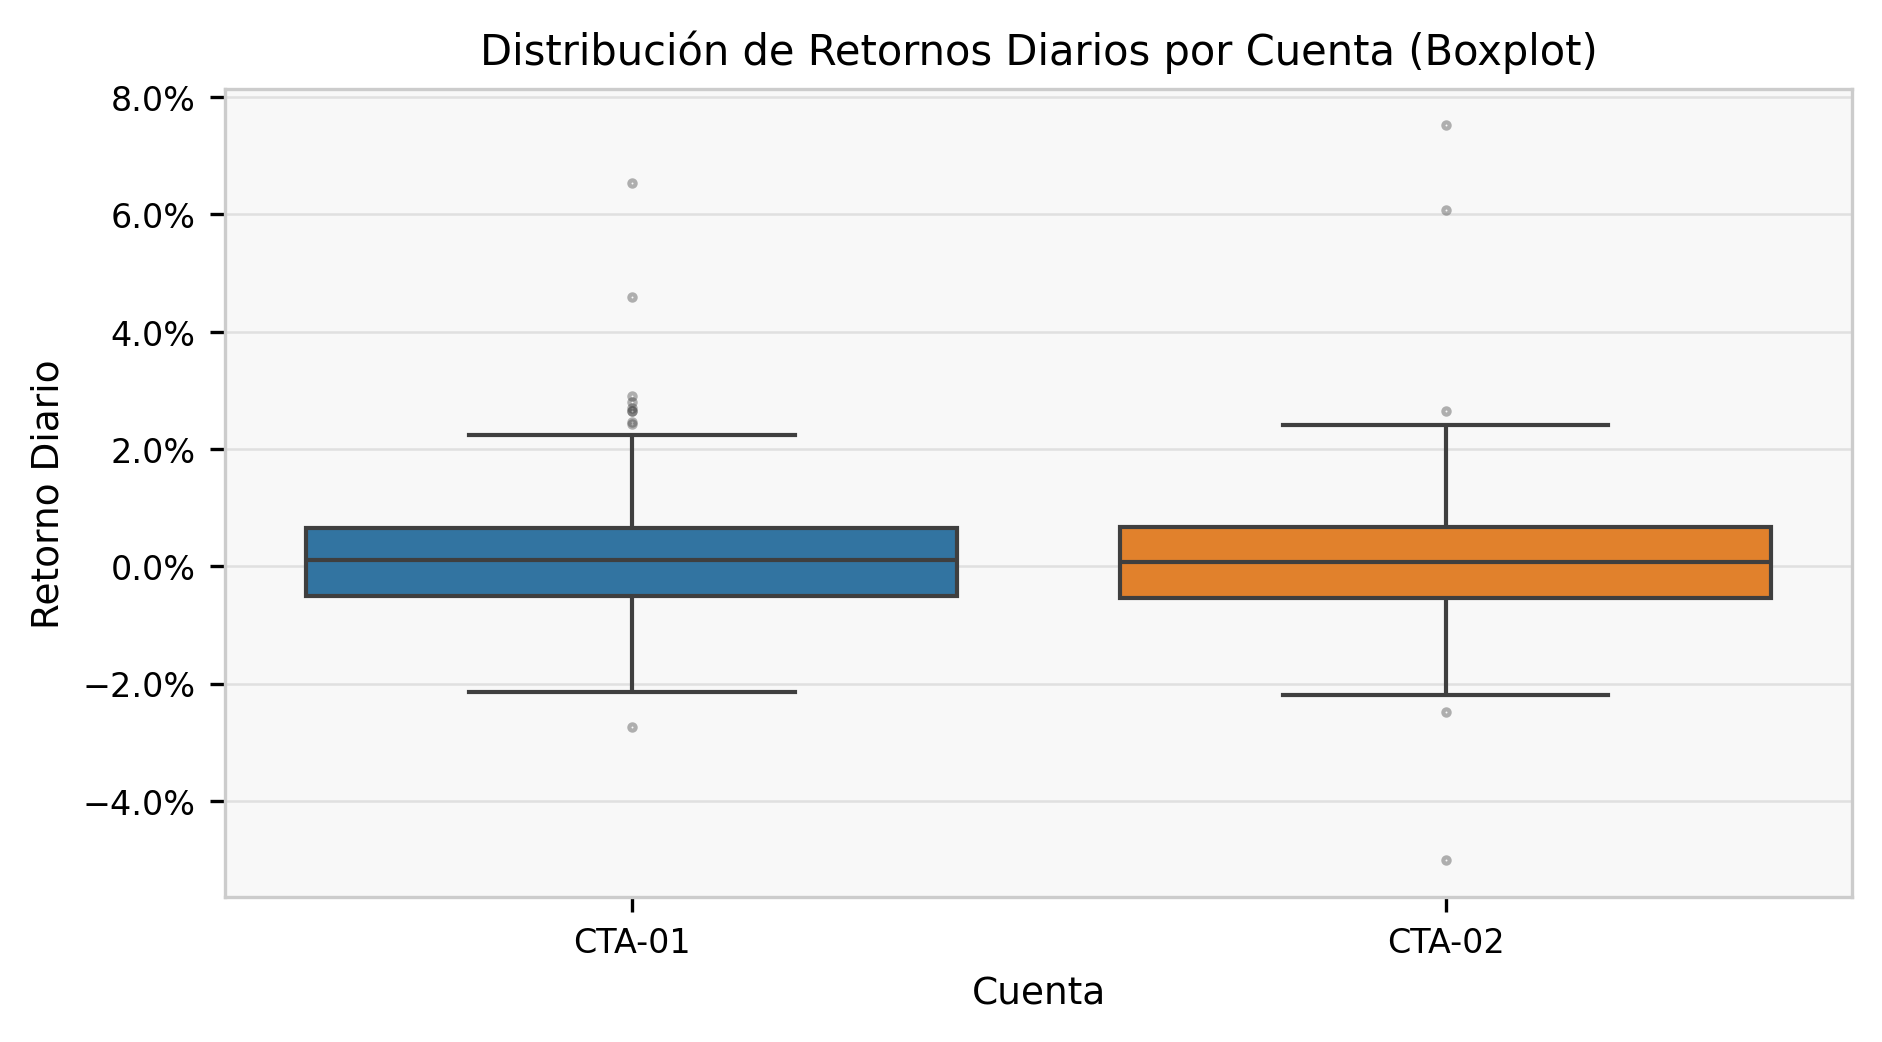
\includegraphics[width=\columnwidth,keepaspectratio]{fig_box_retornos.png}
\caption{Retornos diarios por cuenta (cajas y bigotes).}
\label{fig:box}
\vspace{-2mm}
\end{figure}

% ---- (D) Riesgo en el tiempo
\paragraph{Riesgo en el tiempo.}
La Fig.~\ref{fig:vol} condensa la volatilidad reciente y hace visibles transiciones de régimen; útil para contextualizar episodios de pérdidas/ganancias.
\begin{figure}[!t]
\centering
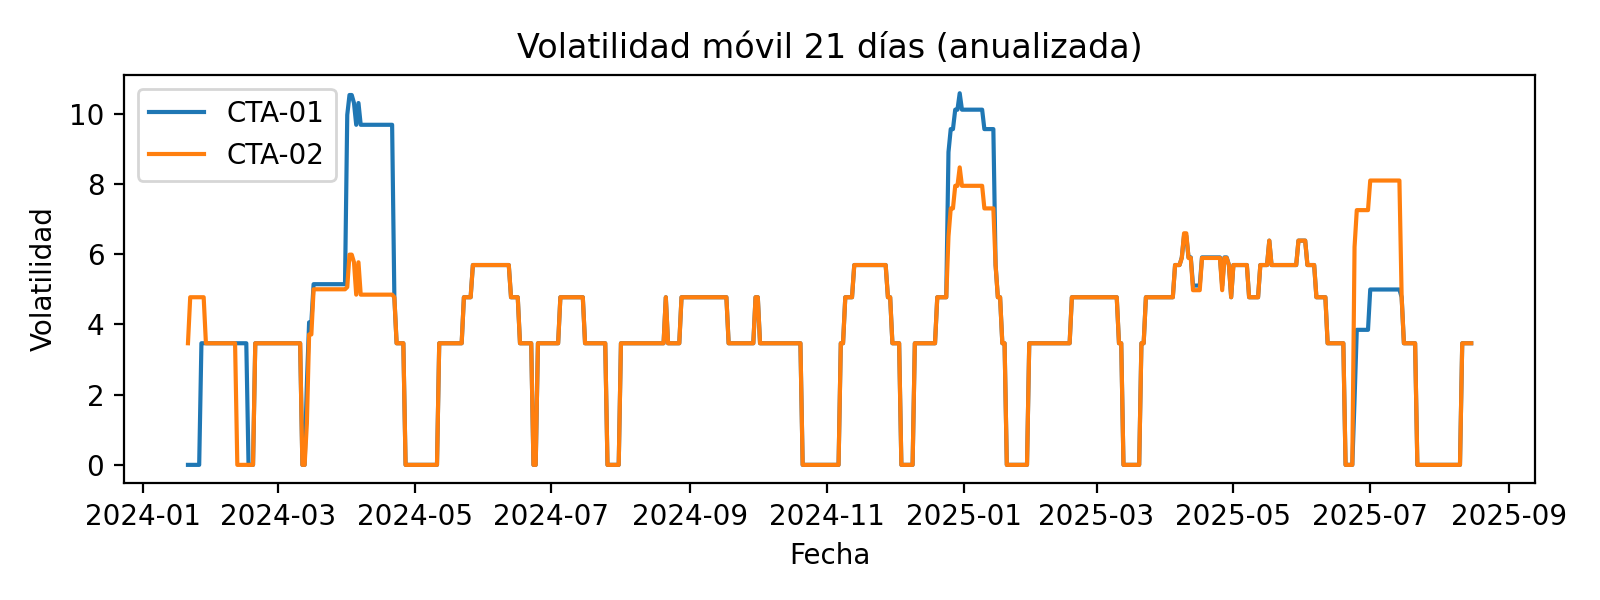
\includegraphics[width=\columnwidth,keepaspectratio]{fig_vol_rolling.png}
\caption{Volatilidad móvil de 21 días (anualizada).}
\label{fig:vol}
\vspace{-2mm}
\end{figure}

% ---- (E) Estacionalidad de retornos
\paragraph{Estacionalidad simple de retornos.}
La Fig.~\ref{fig:mensual} agrega retornos a nivel mensual. Sirve para comunicar ciclos básicos sin introducir estacionalidad compleja.
\begin{figure}[!t]
\centering
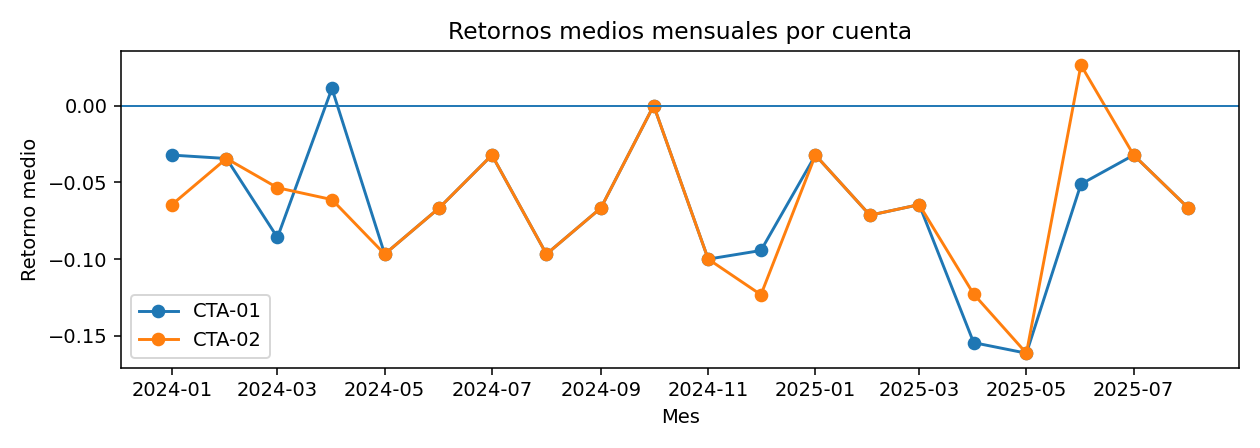
\includegraphics[width=\columnwidth,keepaspectratio]{fig_retornos_mensuales.png}
\caption{Retornos agregados por mes (estacionalidad simple).}
\label{fig:mensual}
\vspace{-2mm}
\end{figure}

% ---- (F) Drawdown y recuperación
\paragraph{\emph{Drawdown} y recuperación.}
La Fig.~\ref{fig:dd} muestra máximas caídas desde picos previos y ayuda a dimensionar “dolor” y tiempo de recuperación.
\begin{figure}[!t]
\centering
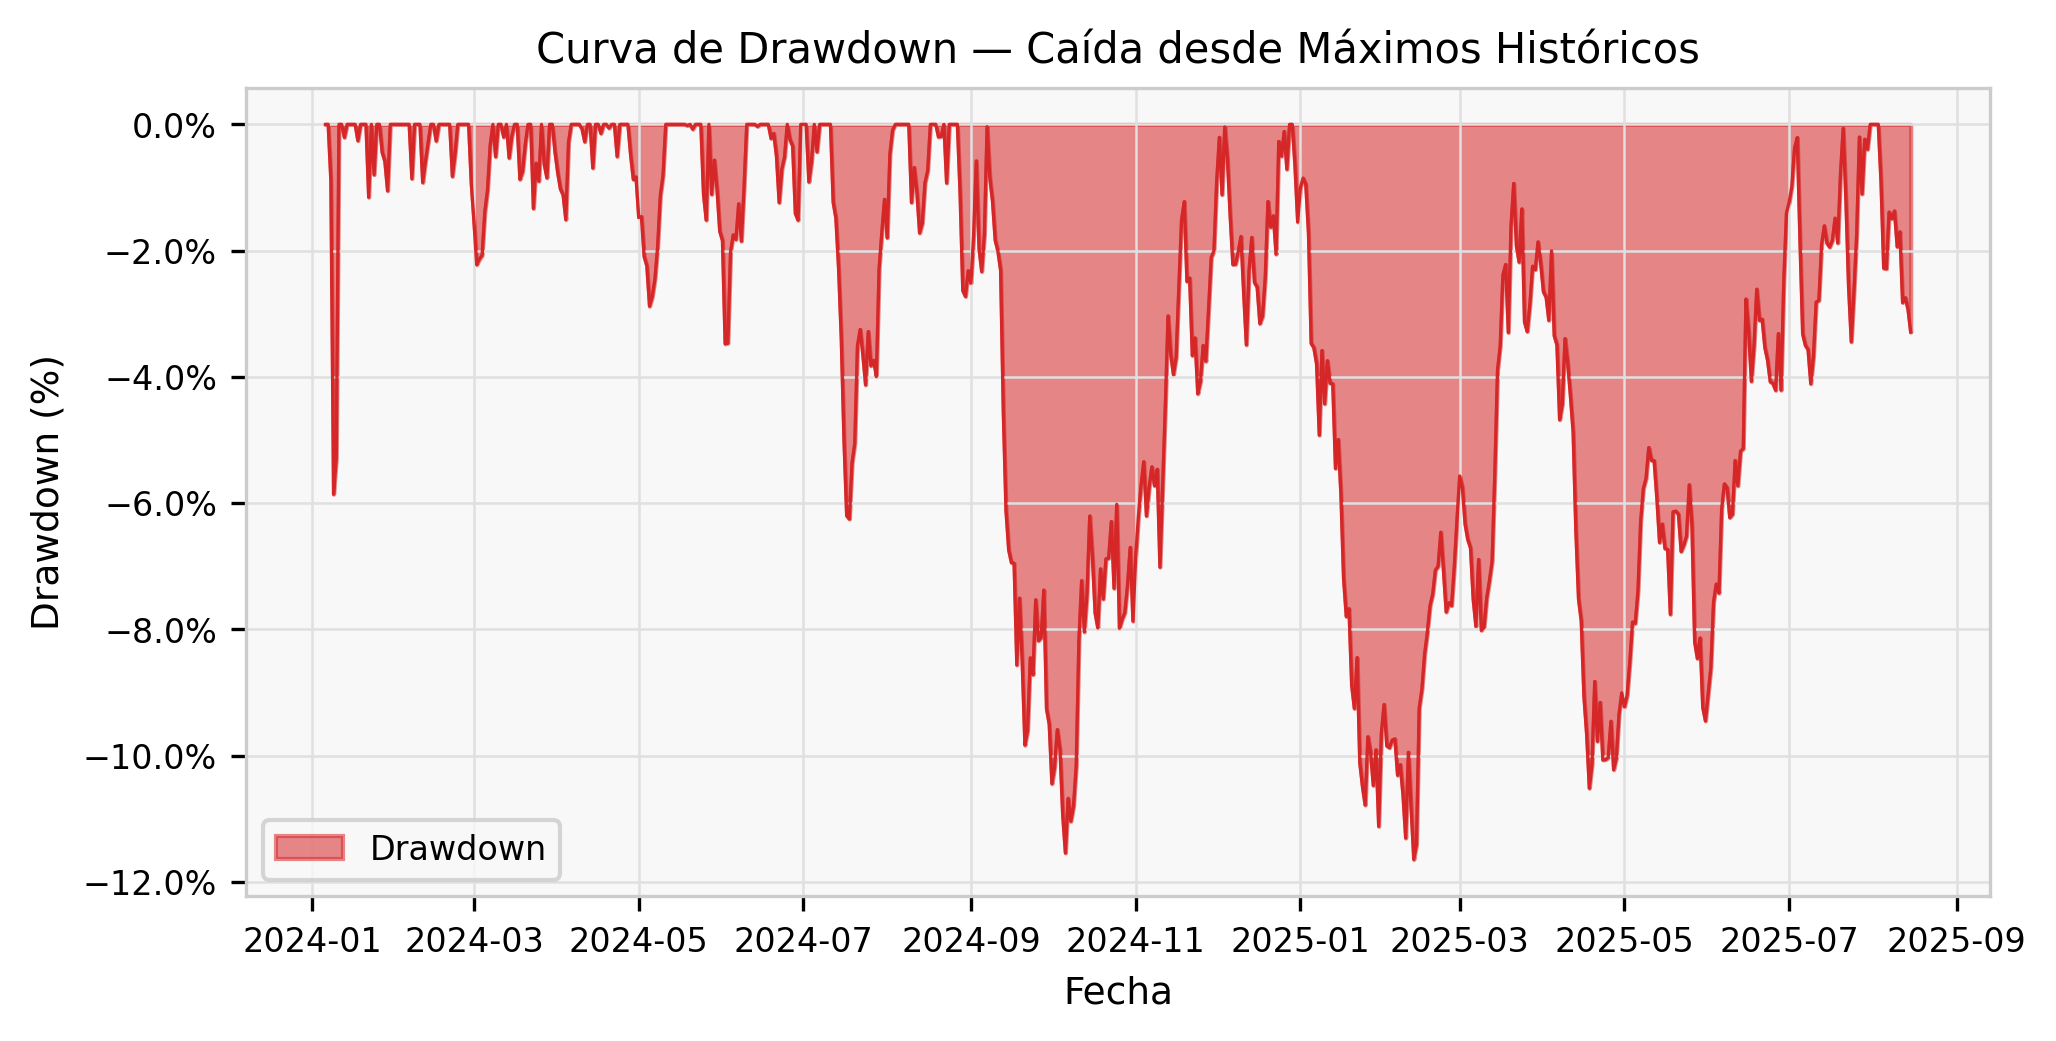
\includegraphics[width=\columnwidth,keepaspectratio]{fig_drawdown.png}
\caption{\emph{Drawdown}: caídas desde máximos previos.}
\label{fig:dd}
\vspace{-2mm}
\end{figure}

% ---- (G) Contribución por activos
\paragraph{Contribución por activos.}
La Fig.~\ref{fig:top10} expone el Top-10 de \emph{tickers} por valor/exposición, focalizando el control donde realmente se mueve la aguja.
\begin{figure}[!t]
\centering
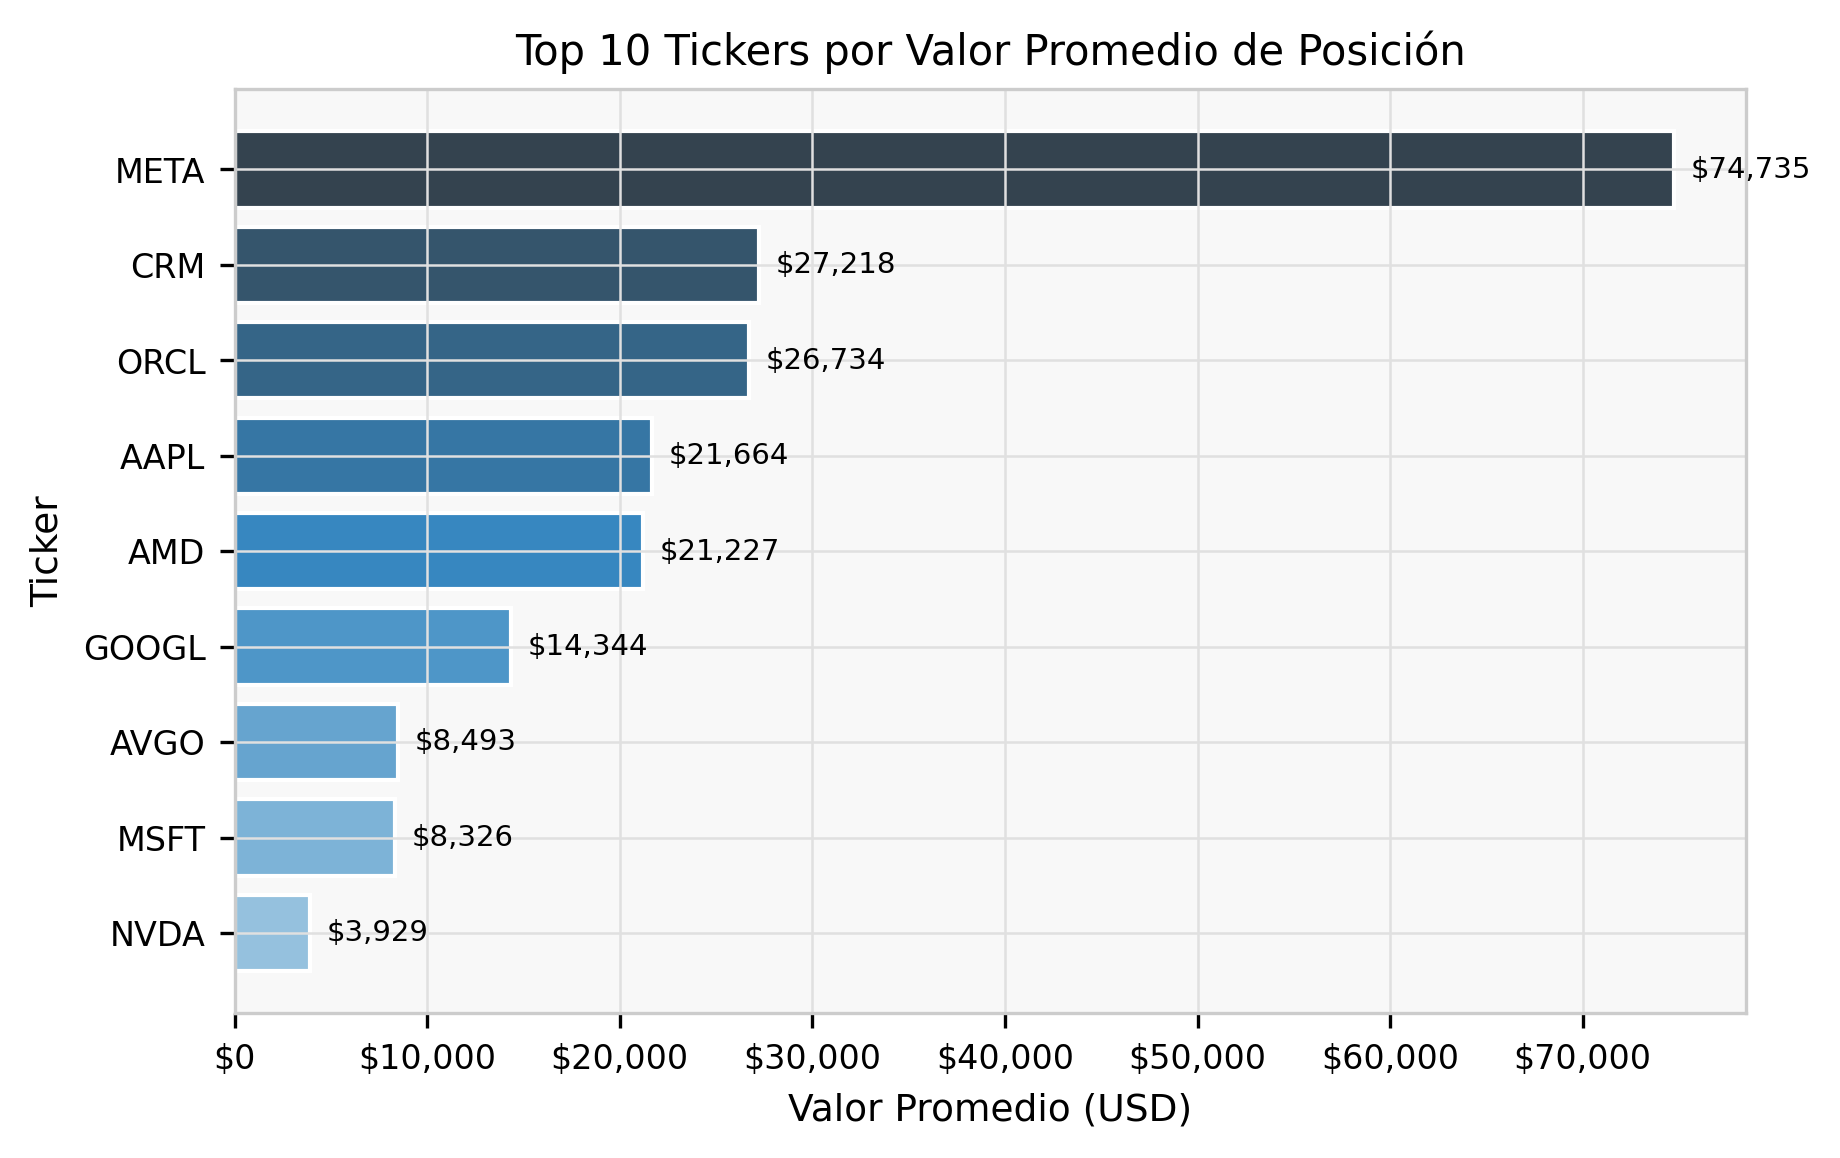
\includegraphics[width=\columnwidth,keepaspectratio]{fig_top10_tickers.png}
\caption{Top-10 de \emph{tickers} por valor/exposición.}
\label{fig:top10}
\vspace{-2mm}
\end{figure}

% ========= 7. Resultados cuantitativos (desde archivos .tex) =========
\section{Resultados cuantitativos}
Para facilitar la auditoría y mantener el documento liviano, las tablas se mantienen en archivos externos y se insertan con \verb|\input|. Esto permite regenerarlas automáticamente desde los CSV y evita errores de copiado.

\subsection{Calidad de datos (DQ\%)}
\begin{table}[!t]
\centering
\caption{Calidad de datos por artefacto (DQ).}
\label{tab:dq2}
\scriptsize
\setlength{\tabcolsep}{3pt}      % menos espacio horizontal entre columnas
\renewcommand{\arraystretch}{1.05}
\begin{tabular}{@{}lrrrrr@{}}
\toprule
\textbf{archivo} & \textbf{registros} & \textbf{válidas \%} & \textbf{dup} & \textbf{clave} & \textbf{inc} \\
\midrule
cartera\_diaria.csv            & 1186  & 100{,}000 & 0 & 0 & 0 \\
benchmark\_vs\_portafolio.csv  & 1145  & 100{,}000 & 0 & 0 & 0 \\
exposicion\_sector.csv         &   10  & 100{,}000 & 0 & 0 & 0 \\
exposicion\_ticker.csv         &   18  & 100{,}000 & 0 & 0 & 0 \\
posiciones\_diarias.csv        & 10674 & 100{,}000 & 0 & 0 & 0 \\
\bottomrule
\end{tabular}
\vspace{-2mm}
\end{table}


\subsection{Latencia y throughput}
\begin{table}[!t]
\centering
\caption{Latencia por etapa del pipeline (5 repeticiones).}
\label{tab:lat}
\resizebox{\columnwidth}{!}{%
\begin{tabular}{@{}lrrl@{}}
\toprule
\textbf{Etapa} & \textbf{t prom (s)} & \textbf{CV (\%)} & \textbf{Hash dataset} \\
\midrule
Extracción CSV & 0{,}003 & 5{,}2 & \texttt{ee1922d0eec8} \\
Transformación & 0{,}002 & 22{,}5 & \texttt{ee1922d0eec8} \\
Exportación    & 0{,}003 & 9{,}9  & \texttt{ee1922d0eec8} \\
\bottomrule
\end{tabular}}
\vspace{-2mm}
\end{table}


\subsection{Escalabilidad (10$\times$--50$\times$)}
\begin{table}
\caption{Pruebas de escalabilidad sintética.}
\label{tab:escala}
\begin{tabular}{lrr}
\toprule
escenario & t\_etl\_s & cv\_\% \\
\midrule
1x & 0.001 & 12.100 \\
10x & 0.004 & 18.900 \\
50x & 0.010 & 2.900 \\
\bottomrule
\end{tabular}
\end{table}


% ========= 8. Verificación de correctitud frente a oráculo =========
\section{Verificación de correctitud frente a un oráculo}
Para asegurar que el ETL produce resultados \emph{correctos} y no sólo consistentes, se compara contra un \textbf{oráculo sencillo} calculado de forma independiente:
\begin{enumerate}
    \item \textbf{Retorno diario por cuenta:} recomputado desde el valor de cartera agregado en $t$ y $t-1$, ignorando días sin valor previo para evitar divisiones por cero.
    \item \textbf{Acumulado:} producto iterativo de $(1+r_t)$ iniciado en el primer día válido de cada cuenta, rebaseado a 1.
    \item \textbf{Brecha vs.\ índice:} diferencia entre el acumulado de la cuenta y el índice rebaseado en cada fecha.
\end{enumerate}
Las diferencias esperadas se acotan a errores de redondeo (puntos base). La Tabla~\ref{tab:oraculo} documenta la comparación (rellenar al ejecutar); si alguna métrica supera el umbral, el reporte DQ marca la corrida como “no publicable” y preserva los artefactos previos.

\begin{table}[!t]
\centering
\caption{Comparación ETL vs.\ oráculo (rellenar al ejecutar)}
\label{tab:oraculo}
\resizebox{\columnwidth}{!}{%
\begin{tabular}{@{}llll@{}}
\toprule
\textbf{Métrica} & \textbf{ETL} & \textbf{Oráculo} & \textbf{Dif.\ (p.b.)} \\
\midrule
Retorno medio diario (\%) & & & \\
Volatilidad 21d (\%) & & & \\
Acumulado fin de periodo & & & \\
Brecha media vs.\ índice (\%) & & & \\
\bottomrule
\end{tabular}}
\vspace{-2mm}
\end{table}

\noindent\textbf{Resultado operativo.} La comparación se integra a \texttt{dq\_resumen.csv} y a un \texttt{.meta.json} por artefacto, habilitando auditorías y pruebas de regresión sin depender del tablero.

% ========= 9. Política de rebalanceo basada en evidencia =========
\section{Política de rebalanceo basada en evidencia}
El tablero no sólo describe el desempeño: habilita decisiones repetibles. Proponemos una política de rebalanceo \emph{liviana} guiada por las vistas ya incluidas (acumulados, volatilidad, donut sectorial y Top-10 de \emph{tickers}).

\subsection{Señales de activación}
\begin{itemize}
    \item \textbf{Riesgo}: la volatilidad móvil de 21 días supera en X p.p. su mediana de 6 meses o aparece una racha de \emph{drawdown} mayor a Y\%.
    \item \textbf{Concentración}: sector con peso $>$ 35\% o \emph{ticker} con peso $>$ 10\% (según Fig.\,\ref{fig:donut} y Fig.\,\ref{fig:top10}).
    \item \textbf{Desempeño relativo}: brecha negativa sostenida vs.\ el índice rebaseado por Z días (Fig.\,\ref{fig:lineas}).
\end{itemize}

\subsection{Acciones prescriptivas}
\begin{itemize}
    \item \textbf{Rebalanceo suave}: recortar 1--3 p.p.\ al sector o \emph{ticker} dominante y redistribuir a los de menor peso dentro del mismo macro–sector.
    \item \textbf{Límites duros}: ningún sector $>$ 40\% y ningún \emph{ticker} $>$ 12\%; reevaluación mensual de límites.
    \item \textbf{Higiene de datos}: si un \emph{ticker} aparece “por homologar”, no aumenta su peso hasta que se corrija el catálogo.
\end{itemize}

\subsection{Plantilla operativa de rebalanceo}
\begin{table}[!t]
\centering
\caption{Plantilla de política de rebalanceo (parametrizable)}
\label{tab:politica}
\resizebox{\columnwidth}{!}{%
\begin{tabular}{@{}lll@{}}
\toprule
\textbf{Condición (señal)} & \textbf{Umbral sugerido} & \textbf{Acción}\\
\midrule
Volatilidad 21d elevada & $>$ mediana 6m + 1\,p.p. & Reducir 2\,p.p. en Top-2 sectores\\
\emph{Drawdown} profundo & $>$ 8\% en 20 días & Pausa compras, revisar liquidez\\
Sector concentrado & $>$ 35\% & Recorte 1--3\,p.p., diversificar\\
\emph{Ticker} concentrado & $>$ 10\% & Limitar a 8--9\%\\
Brecha vs.\ índice & $>$ 3\% (30 días) & Revisar costos y rotación\\
\bottomrule
\end{tabular}}
\vspace{-2mm}
\end{table}

\subsection{Ejemplo guiado}
Con base en el donut sectorial y el Top-10, si “Semiconductores” concentra 41\% y dos \emph{tickers} superan 11\%, se ejecuta un recorte de 2\,p.p.\ al sector y 1\,p.p.\ a cada \emph{ticker} dominante, reasignando a sectores sub–representados. La brecha vs.\ índice y la volatilidad determinan si el ajuste es inmediato o escalonado (dos ventanas semanales).

% ========= 10. Hoja de ruta a producción (SLOs y migración) =========
\section{Hoja de ruta a producción: SLOs, observabilidad y migración}
\subsection{SLOs mínimos}
\begin{itemize}
    \item \textbf{Exactitud numérica:} error absoluto $<$ 2 p.b.\ en métricas validadas por el oráculo.
    \item \textbf{Latencia de refresco:} ETL $<$ 60\,s y actualización de PBI $<$ 15\,s para el conjunto base; $<$ 5\,min a 50$\times$.
    \item \textbf{Disponibilidad:} 99\% de corridas sin fallas por mes académico (excluye caídas externas de Sheets).
\end{itemize}

\subsection{Observabilidad y trazabilidad}
\begin{itemize}
    \item \textbf{Logs estructurados:} un registro por artefacto con \texttt{run\_id}, \texttt{hash}, número de filas, DQ\% y rutas de salida.
    \item \textbf{Alertas:} umbrales para duplicados de clave $>$0, NaN/Inf $>$0 o diferencia vs.\ oráculo $>$2 p.b.
    \item \textbf{Versionado:} carpetas \texttt{out/YYYY-MM/} y enlace firme desde el tablero a la versión publicada.
\end{itemize}

\subsection{Costos y escalamiento}
\begin{itemize}
    \item \textbf{Costo directo:} nulo en Colab/Sheets; PBI Desktop gratuito. En multiusuario, PBI Service añade costo por licencia.
    \item \textbf{Escalamiento simple:} particionado por año/cuenta y carga incremental por archivos; \emph{DirectQuery}/\emph{Direct Lake} como evolución si crece el histórico.
\end{itemize}

\subsection{Migración a microservicios}
\begin{itemize}
    \item \textbf{Ingesta:} API REST para \texttt{/transacciones} y \texttt{/precios} con validación, versión e \emph{idempotency keys}.
    \item \textbf{Procesamiento:} jobs programados (cron/Cloud Scheduler) que ejecutan el ETL y publican artefactos firmados.
    \item \textbf{Presentación:} Power BI capitaliza la ingesta del motor \emph{pyarrow} con Parquet nativo minimizando cuellos de botella semánticos; si se avanza a entornos Delta Lake, el sistema es compatible directamente con \emph{Direct Lake}.
\end{itemize}

% ========= 11. Gobernanza, seguridad y operación =========
\section{Gobernanza, seguridad y operación}
\textbf{Versionado y cambios controlados.} Cada ajuste de esquema se registra en el diccionario y se etiqueta con un \texttt{run\_id}. Los artefactos nuevos conviven con los previos hasta completar la migración del tablero.

\textbf{Privacidad y acceso.} Aunque la publicación como CSV simplifica la ingesta, se recomienda limitar el acceso a “solo con enlace” y rotarlo periódicamente. Para mayor trazabilidad, la arquitectura migra sin fricción a la API oficial de Google con cuenta de servicio y control de permisos.

\textbf{Checklist de salida.} (1) Sin duplicados de clave; (2) fechas en rango; (3) huellas coincidentes; (4) nota breve para cualquier corrección \emph{ad hoc}.

% ========= 12. Amenazas a la validez =========
\section{Amenazas a la validez}
\textbf{Interna.} Decisiones de limpieza (p.~ej., winsorización gráfica) pueden alterar la percepción; por ello, los cálculos conservan los datos completos y las transformaciones estéticas quedan registradas. \\
\textbf{Externa.} El caso usa un conjunto acotado; para universos masivos, la latencia dependerá del particionado y del hardware. \\
\textbf{Constructo.} La varianza captura solo una dimensión del riesgo; conviene añadir métricas de cola y medidas frente a un índice \cite{macias2020,ramirez2016}.

% ========= 13. Conclusiones =========
\section{Conclusiones y trabajo futuro}
Un \emph{stack} mínimo —Sheets, Python y Power~BI— puede entregar resultados coherentes y auditables cuando el proceso está bien especificado. La arquitectura favorece la docencia por su reproducibilidad y constituye una base sólida para prototipos \emph{fintech}. Como evolución: exponer artefactos vía API REST (OAuth2/JWT), programar orquestaciones, incorporar métricas avanzadas (\emph{tracking error}, \emph{information ratio}, medidas de cola) e introducir señales de rebalanceo livianas.

% ========= Bibliografía =========
\bibliographystyle{IEEEtran}
\begin{thebibliography}{00}
\bibitem{zapata2022}
C.\,A. Zapata Quimbayo, ``Modelo Media--Varianza y criterios ASG: de Markowitz al portafolio socialmente responsable,'' \emph{ODEON}, núm.\,21, pp.\,55--79, 2022. DOI: \href{https://doi.org/10.18601/17941113.n21.04}{10.18601/17941113.n21.04}. \emph{(en español)}.
\bibitem{macias2020}
L.\,G. Macías-Trejo, ``La eficiencia media--varianza de un portafolio diversificado entre ISR y un índice de mercado,'' \emph{Estudios Gerenciales}, vol.\,36, no.\,154, 2020. DOI: \href{https://doi.org/10.18046/j.estger.2020.154.3476}{10.18046/j.estger.2020.154.3476}. \emph{(en español)}.
\bibitem{ramirez2016}
N. Ramírez Carmona y O. García Salgado, ``Estado del arte en teoría de portafolios: del análisis individual de acciones a la optimización multiobjetivo,'' \emph{Economía Coyuntural}, vol.\,1, no.\,4, pp.\,101--144, 2016. Disponible en: \url{http://www.scielo.org.bo/scielo.php?script=sci_arttext&pid=S2415-06222016000400005}. \emph{(en español)}.
\bibitem{barbosa2019}
M.\,I. Barbosa Camargo, A. Salazar Sarmiento y K.\,J. Peñaloza Gómez, ``Valoración de riesgo mediante modelos GARCH y simulación Montecarlo: evidencia del mercado accionario colombiano,'' \emph{Semestre Económico}, vol.\,22, no.\,53, pp.\,53--75, 2019. DOI: \href{https://doi.org/10.22395/seec.v22n53a3}{10.22395/seec.v22n53a3}. \emph{(en español)}.
\bibitem{gaona2020}
F. Gaona Montiel, A. Reyes Robles y E. Ramírez Cedillo, ``Mercados, volatilidad y gestión de futuros en México: el empleo del método ARCH y GARCH,'' \emph{Contaduría y Administración}, vol.\,65, no.\,1, e150, 2020. DOI: \href{https://doi.org/10.22201/fca.24488410e.2018.1752}{10.22201/fca.24488410e.2018.1752}. \emph{(en español)}.
\bibitem{novoa2019}
N. Novoa-Torres, D.\,R. Bermúdez-Huérfano y H. Zamora-Carrillo, ``Nociones, consideraciones y ventajas de la inteligencia de negocios (BI),'' \emph{Revista Vínculos}, vol.\,16, no.\,2, pp.\,280--287, 2019. DOI: \href{https://doi.org/10.14483/2322939X.15592}{10.14483/2322939X.15592}. \emph{(en español)}.
\end{thebibliography}

\end{document}
